\chapter{Экспериментальный раздел}
\label{cha:research}
    В данном разделе будут проведены эксперименты для проведения 
    сравнительного анализа алгоритмов по затрачиваемому процессорному 
    времени в зависимости от длины массива и степени его отсортированности.

    \section{Сравнительный анализ на основе замеров времени работы алгоритмов}
        В рамках данного проекта были проведёны следующие эксперименты:

        1) сравнение времени работы сортировок в лучшем случае(график \ref{graph:test:1});
        
        2) сравнение времени работы сортировок в худшем случае(график \ref{graph:test:2}).

        3) сравнение времени работы сортировок в произвольном случае(график \ref{graph:test:3}).
        
        Тестирование проводилось на компьютере с процессором
        Intel(R) Core(TM) i5-8265U CPU @ 1.60GHz 1.80 GHz под управлением Windows 11 с 8 Гб оперативной памяти.\\

        \begin{figure}[h!]
            \centering
            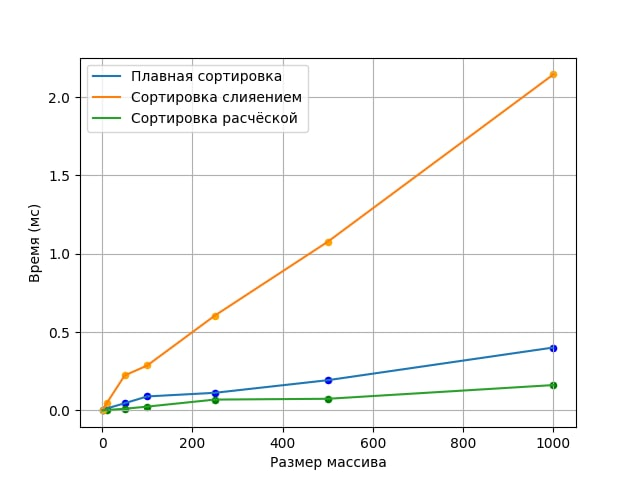
\includegraphics[scale=0.9]{graph_1.png}
            \caption{Зависимость времени работы алгоритмов от размера массива в лучшем случае}
            \label{graph:test:1}
        \end{figure}
        \newpage
        \begin{figure}[h!]
            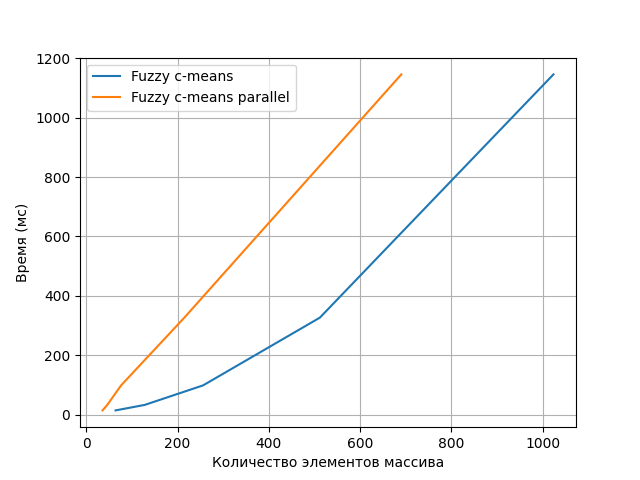
\includegraphics[scale=0.9]{graph_2.png}
            \caption{Зависимость времени работы алгоритмов от размера массива в худшем случае}
            \label{graph:test:2}
        \end{figure}
        \newpage
        \begin{figure}[h!]
            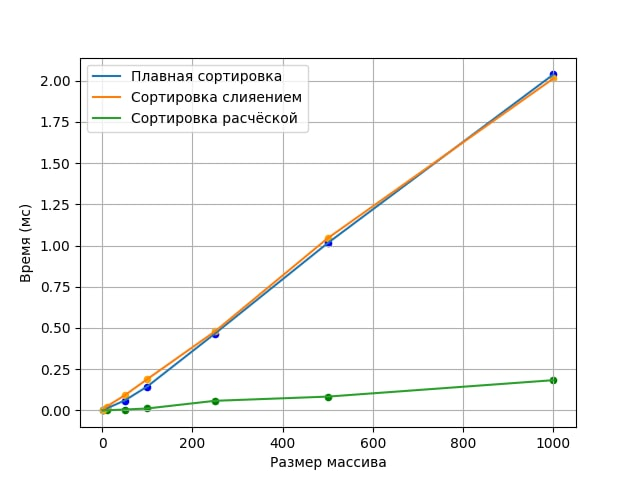
\includegraphics[scale=0.9]{graph_3.png}
            \caption{Зависимость времени работы алгоритмов от размера массива в произвольном случае}
            \label{graph:test:3}
        \end{figure}



    \section{Вывод}
        \par В ходе экспериментов по замеру времени работы было установлено, что в лучшем случае, когда массив отсортирован, сортировка слиянием оказалась самой медленной.
        \par В худшем случае сортировка слиянием и плавная сортировка работают одинаково хуже сортировки расчёской.
        \par В произвольном случае время работы сортировок слияением и плавной сортировки сопоставимо.
        Сортировка расчёской работает одинаково хорошо во всех случаях.


\newpage